\subsection{Vehicles}

In our autonomous intersection model, there were originally two types of vehicles that were defined: autonomous vehicles and human driven vehicles.  However, given the scope of the project, the vehicle types were reduced to autonomous vehicles only. The autonomous vehicles all take on the same physical characteristics in our model. These properties are explained in the following section.

\subsubsection{Vehicle Model Properties}

Typically, cars are classified into many different phycial categories.  For simplicity, our model utilizes the most common type of vehicle, the passenger car (denoted as type P vehicle).  We define vehicle characteristics based on the intersection properties, normally defined in local roadway laws and regulations.  In this project, minimum characteristics of type P cars require a minimum inside radius of 16 ft. from the inner edge of the lane \cite{Bureau}.  This is implemented in our model in the pathway equations.  In our model, vehicles have certain properties that are similar to those seen in the physical world.  Exceptions have been made to make the simulation tractible and because these exceptions are reasonable within the given model.  First, we model vehicles with the ability to instantaneously change velocity and place a requirement that they have a constant velocity within intersection.  All intersection route paths are 68 ft or less and allow for limited change in velocity in the physical world.  Because of this, a constant velocity model is reasonable.

Another property is that range of the constant velocity of each car must be between 20-40 MPH: $V \rightarrow V \in [20,40]$ \cite{Motorists}.  In the model, the velocity is randomly generated within this range, simulating cars entering the model at different speeds.  These speeds are seen in intersection documentation and are directly implemented into the vehicle properties. Vehicle entry times and route are also randomly generated in order to simulate the authentic intersection.  We require routes to be constant throughout intersection traversal; this follows from standard intersection traffic laws.  The route is randomly generated from two parameters: path and direction.  The direction parameter determines which direction (North, South, East, or West) that the car will enter from, and the path parameter defines which path the vehicle will take (left turn, straight from left lane, straight from right lane, or right turn) from the given direction.  These randomly generated parameters describe the car speed, entry time, and route in our model.

To implement our model, we used Ptolemy II.  Ptolemy limitations prevent dynamic instantiation of new actors during simulation.  This presented a challenge as an intersection model needs continuous vehicle flow.  In order to overcome this, we use the Multi-Instance Composite Actor to emulate dynamic instantiation.  The Multi-Instance Composite Actor allows for $N$ instances of the vehicle modal model within this actor.  Each modal model represents a vehicle that may be in the intersection.  The number of vehicles in the intersection at any given time is limited to, at most, $N$ vehicles.  Vehicles exit the system when their travelled distance is greater than the distance of the given route that they are assigned.  The simulation then regenerates new parameters for the car and a new entry time in which the car can re-enter the intersection, thus effectively creating continuous vehicle flow. The following figure shows a high level view of the overal system.

\begin{center}
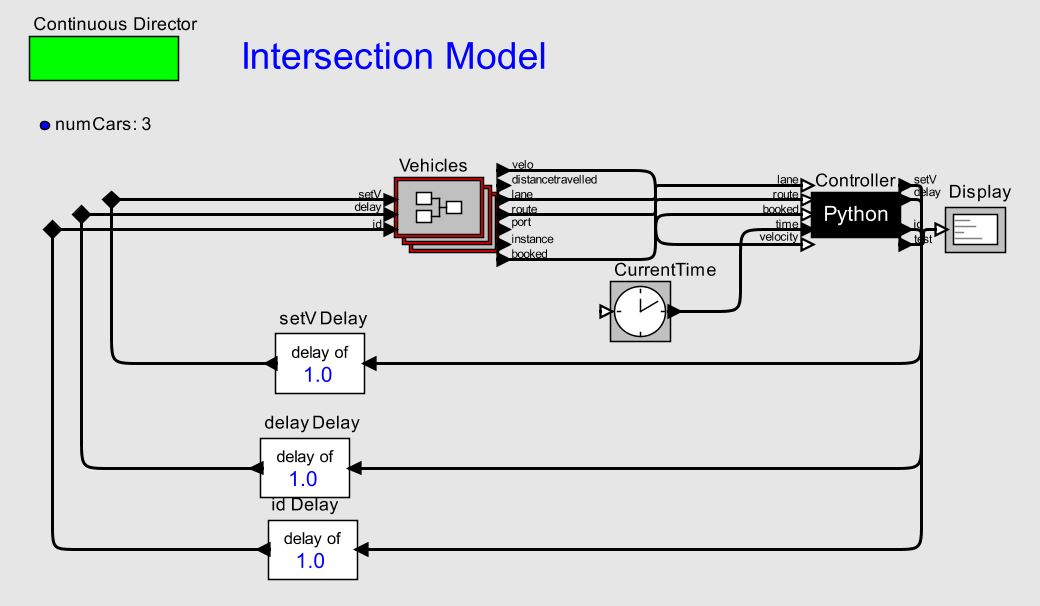
\includegraphics[width=0.65\linewidth]{diagram/ptolemy_system.jpg}
\end{center}

Within each instance of the Multi-Instance Composite Actor, there exist the random parameter generators as well as the modal model that houses the FSM Actor.  This can be seen below:
\begin{center}
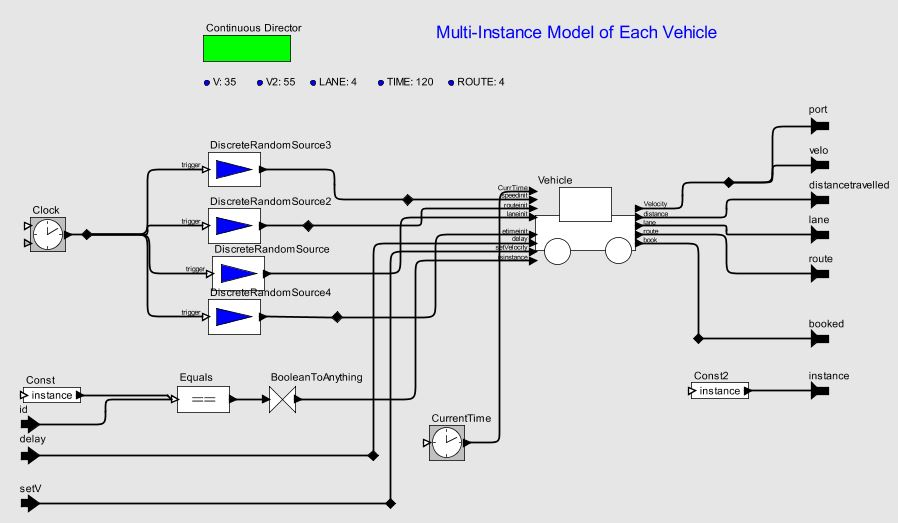
\includegraphics[width=0.65\linewidth]{diagram/ptolemy_multiinstance_actor.jpg}
\end{center}

Finally, there is the Modal Model.  This is a FSM Actor that contains the following states: \texttt{RUN, IDLE, ENTER, BOOK, GO,} and \texttt{WAIT}.  The \texttt{RUN} and \texttt{IDLE} states initialize the parameters of the vehicle and effectively instantiate a vehicle.  The car receives an initial route and velocity and waits in the \texttt{IDLE} state until its entry time has occurred.  Once the entry time has passed, the vehicle is in the \texttt{ENTER} state.  This state represents a vehicle entering the straightaway path before the intersection itself.  Given the vehicle's speed, the model calculates the time at which the vehicle will enter the intersection and sends this to the controller along with its route, speed, and instance.  The controller can then book the vehicle instance in this state, assigning it a different speed, a delay time at the intersection, or no command at all.  If a vehicle reaches the intersection (i.e. global time is greater than the time calculated in the straightaway), then we require that the vehicle stop at the intersection until it is booked.  Once a vehicle is booked (regardless of whether or not it has arrived at the intersection), it enters the \texttt{BOOK} state.  Here it waits until global time exceeds the straightaway time and then proceeds to the \texttt{GO} state.  This state models the vehicle going through the intersection itself, and outputs the distance travelled as well as the current velocity.  Once the vehicle has travelled the specified distance determined by its route, it goes to the \texttt{WAIT} state where the vehicle is set up for initialization again.  This loop continues as long as the simulation is running.  The FSM states can be seen in the following image:
\begin{center}
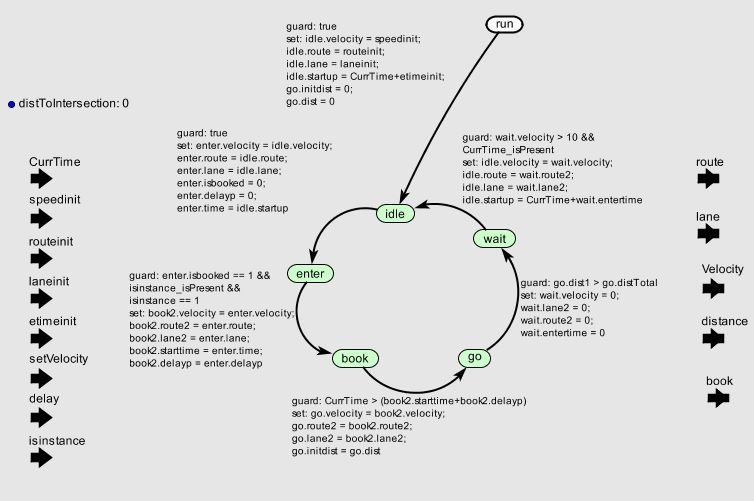
\includegraphics[width=0.65\linewidth]{diagram/ptolemy_vehicle_fsm.jpg}
\end{center}

